% Gerado por tools/qualitative_examples.py; \erro marca palavra que difere da referência.
\providecommand{\erro}[1]{\underline{#1}}

% --- v6_fixes_others_miss: The recognizer erred, v6 gets the line right, and at least two of A, B, C still err.
\noindent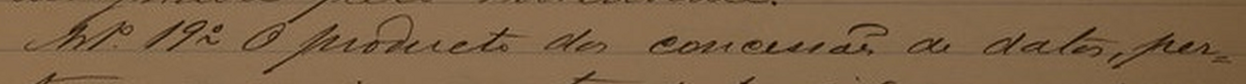
\includegraphics[width=\linewidth]{crops/test10_p23_l024.png}\\[2pt]
{\footnotesize\begin{tabular}{@{}lp{0.68\linewidth}r@{}}
\toprule
referência (normalizada) & art º 19 º o producto das concessões de datas pertence & erros \\
\midrule
sem pós-correção & \erro{Art.º} \erro{19.º} O producto das concessões de datas, \erro{per=} & 1 \\
\textbf{v6 (nossa)} & \erro{Art.º} \erro{19.º} O producto das concessões de datas, pertence & 0 \\
A: KenLM & \erro{Art.º} \erro{19.º} O producto das concessões de datas, pertence & 0 \\
B: \textit{word beam} & \erro{art.º} \erro{19.º} o producto das concessões de datas, \erro{pertece} & 1 \\
C: ByT5 & \erro{Art.º} \erro{19.º} O producto das concessões de datas, \erro{pervence} & 1 \\
D: v6 + PortOldBERT & \erro{Art.º} \erro{19.º} O producto das concessões de datas, pertence & 0 \\
E: VLM & \erro{Art.º} \erro{19.º} O \erro{produto} das concessões de datas, perTence & 1 \\
\bottomrule
\end{tabular}}\\[-2pt]
{\scriptsize página 23 (teste), linha 25}

\noindent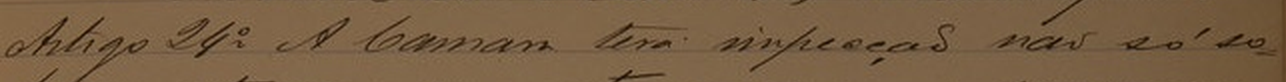
\includegraphics[width=\linewidth]{crops/test10_p25_l001.png}\\[2pt]
{\footnotesize\begin{tabular}{@{}lp{0.68\linewidth}r@{}}
\toprule
referência (normalizada) & artigo 24 º a camara terá inspecção não só sobre & erros \\
\midrule
sem pós-correção & Artigo \erro{24.º} A Camara terá \erro{impecção} não só \erro{so=} & 2 \\
\textbf{v6 (nossa)} & Artigo \erro{24.º} A Camara terá inspecção não só sobre & 0 \\
A: KenLM & Artigo \erro{24.º} A Camara terá \erro{inpecção} não só sobre & 1 \\
B: \textit{word beam} & artigo \erro{24.º} a camara terá \erro{inpecção} não só sobre & 1 \\
C: ByT5 & Artigo \erro{24.º} A Camara terá \erro{impecção} não só \erro{sosobre} & 2 \\
D: v6 + PortOldBERT & Artigo \erro{24.º} A Camara terá inspecção não só sobre & 0 \\
E: VLM & Artigo \erro{24.º} A \erro{Câmara} terá \erro{inspeção} não só & 3 \\
\bottomrule
\end{tabular}}\\[-2pt]
{\scriptsize página 25 (teste), linha 2}

\noindent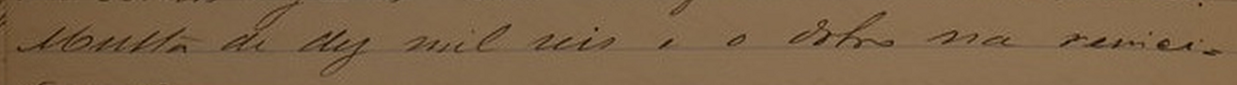
\includegraphics[width=\linewidth]{crops/test10_p44_l002.png}\\[2pt]
{\footnotesize\begin{tabular}{@{}lp{0.68\linewidth}r@{}}
\toprule
referência (normalizada) & multa de dez mil reis e o dobro na reincidencia & erros \\
\midrule
sem pós-correção & Multa de dez mil reis e o dobro na \erro{reinci=} & 1 \\
\textbf{v6 (nossa)} & Multa de dez mil reis e o dobro na reincidencia. & 0 \\
A: KenLM & Multa de dez mil reis e o dobro na reincidencia. & 0 \\
B: \textit{word beam} & multa de dez mil reis e o dobro na \erro{reineidencia} & 1 \\
C: ByT5 & Multa de dez mil reis e o dobro na \erro{reincidendencia.} & 1 \\
D: v6 + PortOldBERT & Multa de dez mil reis e o dobro na reincidencia. & 0 \\
E: VLM & Multa de dez mil reis e o dobro na \erro{reincidência} & 1 \\
\bottomrule
\end{tabular}}\\[-2pt]
{\scriptsize página 44 (teste), linha 3}

\noindent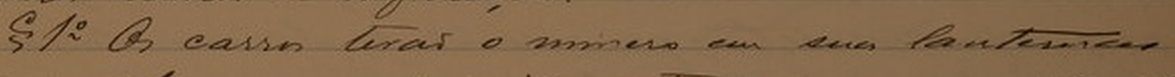
\includegraphics[width=\linewidth]{crops/test10_p55_l013.png}\\[2pt]
{\footnotesize\begin{tabular}{@{}lp{0.68\linewidth}r@{}}
\toprule
referência (normalizada) & 1 º os carros terão o numero em suas lanternas & erros \\
\midrule
sem pós-correção & § \erro{1.º} Os carros terão o \erro{miiero} em suas \erro{lanterinzes} & 2 \\
\textbf{v6 (nossa)} & § \erro{1.º} Os carros terão o numero em suas lanternas & 0 \\
A: KenLM & § \erro{1.º} Os carros terão o numero em suas \erro{lanterinzes} & 1 \\
B: \textit{word beam} & § \erro{1.º} os carros terão o \erro{mero} em suas lanternas & 1 \\
C: ByT5 & § \erro{1.º} Os carros terão o \erro{minimo} em suas \erro{lanterinas} & 2 \\
D: v6 + PortOldBERT & § \erro{1.º} Os carros terão o numero em suas lanternas & 0 \\
E: VLM & § \erro{1.º} Os carros terão o \erro{miiero} em suas lanternas & 1 \\
\bottomrule
\end{tabular}}\\[-2pt]
{\scriptsize página 55 (teste), linha 14}

% --- vlm_modernizes: The recognizer already read the line right; v6 keeps it; the VLM introduces errors.
\noindent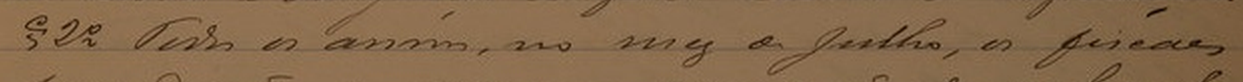
\includegraphics[width=\linewidth]{crops/test10_p55_l016.png}\\[2pt]
{\footnotesize\begin{tabular}{@{}lp{0.68\linewidth}r@{}}
\toprule
referência (normalizada) & 2 º todos os annos no mez de julho os fiscaes & erros \\
\midrule
sem pós-correção & § \erro{2.º} Todos os annos, no mez de Julho, os fiscaes & 0 \\
\textbf{v6 (nossa)} & § \erro{2.º} Todos os annos, no mez de Julho, os fiscaes & 0 \\
A: KenLM & § \erro{2.º} Todos os annos, no mez de Julho, os fiscaes & 0 \\
B: \textit{word beam} & § \erro{2.º} todos os annos, no mez de julho, os fiscaes & 0 \\
C: ByT5 & § \erro{2.º} Todos os annos, no mez de Julho, os fiscaes & 0 \\
D: v6 + PortOldBERT & § \erro{2.º} Todos os annos, no mez de Julho, os fiscaes & 0 \\
E: VLM & § \erro{2.º} Todos os \erro{anos,} no \erro{mês} de Julho, os \erro{fiscais} & 3 \\
\bottomrule
\end{tabular}}\\[-2pt]
{\scriptsize página 55 (teste), linha 17}

\noindent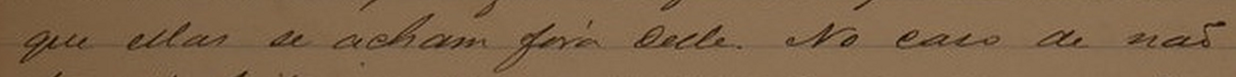
\includegraphics[width=\linewidth]{crops/test10_p18_l003.png}\\[2pt]
{\footnotesize\begin{tabular}{@{}lp{0.68\linewidth}r@{}}
\toprule
referência (normalizada) & que ellas se acham fóra delle no caso de não & erros \\
\midrule
sem pós-correção & que ellas se acham fóra delle. No caso de não & 0 \\
\textbf{v6 (nossa)} & que ellas se acham fóra delle. No caso de não & 0 \\
A: KenLM & que ellas se acham fóra delle. No caso de não & 0 \\
B: \textit{word beam} & que ellas se acham fóra delle. no caso de não & 0 \\
C: ByT5 & que ellas se acham fóra delle. No caso de não & 0 \\
D: v6 + PortOldBERT & que ellas se acham fóra delle. No caso de não & 0 \\
E: VLM & que ellas se acham \erro{fora} \erro{delas.} No caso de não & 2 \\
\bottomrule
\end{tabular}}\\[-2pt]
{\scriptsize página 18 (teste), linha 4}

\noindent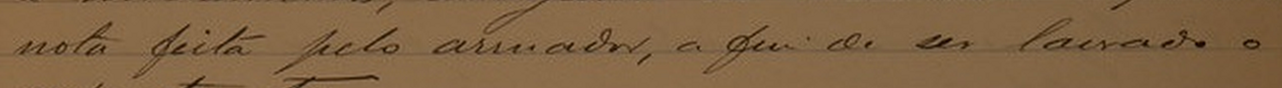
\includegraphics[width=\linewidth]{crops/test10_p31_l004.png}\\[2pt]
{\footnotesize\begin{tabular}{@{}lp{0.68\linewidth}r@{}}
\toprule
referência (normalizada) & nota feita pelo arruador a fim de ser lavrado o & erros \\
\midrule
sem pós-correção & nota feita pelo arruador, a fim de ser lavrado o & 0 \\
\textbf{v6 (nossa)} & nota feita pelo arruador, a fim de ser lavrado o & 0 \\
A: KenLM & nota feita pelo arruador, a fim de ser lavrado o & 0 \\
B: \textit{word beam} & nota feita pelo arruador, a fim de ser lavrado o & 0 \\
C: ByT5 & nota feita pelo arruador, a fim de ser lavrado o & 0 \\
D: v6 + PortOldBERT & nota feita pelo arruador, a fim de ser lavrado o & 0 \\
E: VLM & nota feita pelo \erro{aruador,} a fim de ser lavrado o & 1 \\
\bottomrule
\end{tabular}}\\[-2pt]
{\scriptsize página 31 (teste), linha 5}

\noindent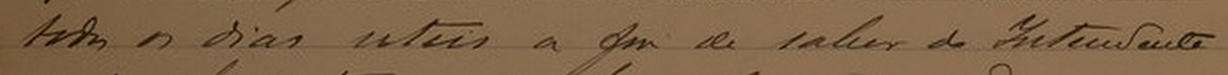
\includegraphics[width=\linewidth]{crops/test10_p32_l019.png}\\[2pt]
{\footnotesize\begin{tabular}{@{}lp{0.68\linewidth}r@{}}
\toprule
referência (normalizada) & todos os dias uteis a fim de saber do intendente & erros \\
\midrule
sem pós-correção & todos os dias uteis a fim de saber do Intendente & 0 \\
\textbf{v6 (nossa)} & todos os dias uteis a fim de saber do Intendente & 0 \\
A: KenLM & todos os dias uteis a fim de saber do Intendente & 0 \\
B: \textit{word beam} & todos os dias uteis a fim de saber do intendente & 0 \\
C: ByT5 & todos os dias uteis a fim de saber do Intendente & 0 \\
D: v6 + PortOldBERT & todos os dias uteis a fim de saber do Intendente & 0 \\
E: VLM & todos os dias \erro{úteis} a fim de saber do Intendente & 1 \\
\bottomrule
\end{tabular}}\\[-2pt]
{\scriptsize página 32 (teste), linha 20}

% --- byt5_better: ByT5 beats v6 on the line (the numeral / split-merge cases v6 cannot reach).
\noindent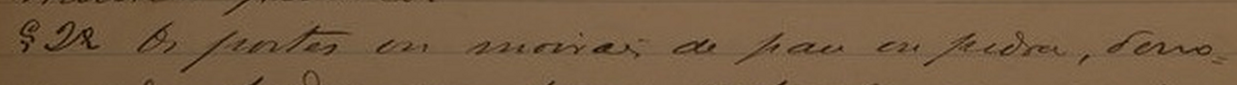
\includegraphics[width=\linewidth]{crops/test10_p22_l029.png}\\[2pt]
{\footnotesize\begin{tabular}{@{}lp{0.68\linewidth}r@{}}
\toprule
referência (normalizada) & º os postes ou moirões de pau ou pedra denominados & erros \\
\midrule
sem pós-correção & § \erro{2º} Os postes ou moirões de pau ou pedra, \erro{deno=} & 2 \\
\textbf{v6 (nossa)} & § \erro{2º} Os postes ou \erro{moitões} de pau ou pedra, \erro{consummados} & 3 \\
A: KenLM & § \erro{28} Os postes ou moirões de pau ou pedra, \erro{donorimados} & 2 \\
B: \textit{word beam} & § \erro{2º} os postes ou moirões de pau ou pedra, \erro{donorimados} & 2 \\
C: ByT5 & § \erro{2.º} Os postes ou moirões de pau ou pedra, \erro{denonumados} & 2 \\
D: v6 + PortOldBERT & § \erro{2º} Os postes ou \erro{moitões} de pau ou pedra, \erro{consummados} & 3 \\
E: VLM & § \erro{2º} Os postes ou moirões de pau ou pedra, \erro{denonmiados} & 2 \\
\bottomrule
\end{tabular}}\\[-2pt]
{\scriptsize página 22 (teste), linha 30}

\noindent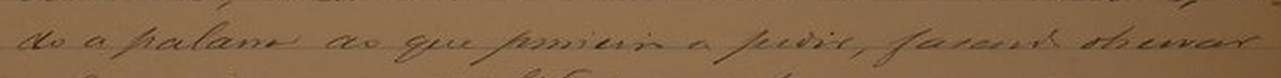
\includegraphics[width=\linewidth]{crops/heldout_p07_l020.png}\\[2pt]
{\footnotesize\begin{tabular}{@{}lp{0.68\linewidth}r@{}}
\toprule
referência (normalizada) & a palavra ao que primeiro a pedir fazendo observar & erros \\
\midrule
sem pós-correção & \erro{do} a \erro{palarra} ao que primeiro a pedir, fazendo \erro{obseovar} & 3 \\
\textbf{v6 (nossa)} & a palavra \erro{do} que primeiro a pedir, fazendo observar & 1 \\
A: KenLM & a palavra \erro{do} que primeiro a pedir, fazendo observar & 1 \\
B: \textit{word beam} & a palavra ao que primeiro a pedir, fazendo observar & 0 \\
C: ByT5 & a palavra ao que primeiro a pedir, fazendo observar & 0 \\
D: v6 + PortOldBERT & a palavra \erro{do} que primeiro a pedir, fazendo observar & 1 \\
E: VLM & a palavra ao que primeiro a pedir, fazendo observar & 0 \\
\bottomrule
\end{tabular}}\\[-2pt]
{\scriptsize página 7 (reservadas), linha 21}

\noindent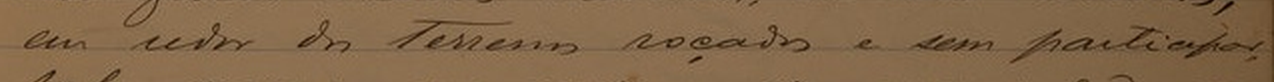
\includegraphics[width=\linewidth]{crops/test10_p55_l025.png}\\[2pt]
{\footnotesize\begin{tabular}{@{}lp{0.68\linewidth}r@{}}
\toprule
referência (normalizada) & em redor dos terrenos roçados e sem participar pelo & erros \\
\midrule
sem pós-correção & em redor dos terrenos roçados e sem \erro{partiaipar=} & 2 \\
\textbf{v6 (nossa)} & em redor dos terrenos roçados e sem \erro{participarem} & 2 \\
A: KenLM & em redor dos terrenos roçados e sem \erro{participarpelo} & 2 \\
B: \textit{word beam} & em redor dos terrenos roçados e sem \erro{participarpelo} & 2 \\
C: ByT5 & em redor dos terrenos roçados e sem participar & 1 \\
D: v6 + PortOldBERT & em redor dos terrenos roçados e sem \erro{participarem} & 2 \\
E: VLM & em redor dos terrenos roçados e sem participar & 1 \\
\bottomrule
\end{tabular}}\\[-2pt]
{\scriptsize página 55 (teste), linha 26}

\noindent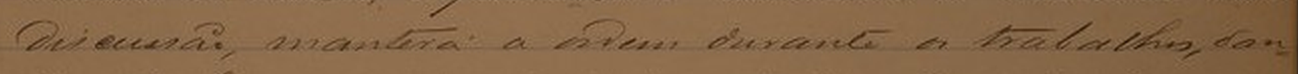
\includegraphics[width=\linewidth]{crops/heldout_p07_l019.png}\\[2pt]
{\footnotesize\begin{tabular}{@{}lp{0.68\linewidth}r@{}}
\toprule
referência (normalizada) & discussão manterá a ordem durante os trabalhos dando & erros \\
\midrule
sem pós-correção & discussão, manterá a ordem durante os trabalhos, \erro{dan=} & 1 \\
\textbf{v6 (nossa)} & discussão, manterá a ordem durante os trabalhos, \erro{dado} & 1 \\
A: KenLM & discussão, manterá a ordem durante os trabalhos, dando & 0 \\
B: \textit{word beam} & discussão, manterá a ordem durante os trabalhos, dando & 0 \\
C: ByT5 & discussão, manterá a ordem durante os trabalhos, dando & 0 \\
D: v6 + PortOldBERT & discussão, manterá a ordem durante os trabalhos, \erro{dado} & 1 \\
E: VLM & discussão, manterá a ordem durante os trabalhos, dando & 0 \\
\bottomrule
\end{tabular}}\\[-2pt]
{\scriptsize página 7 (reservadas), linha 20}

% --- v6_breaks: v6 makes the line worse than the raw recognizer output (a v6 failure case).
\noindent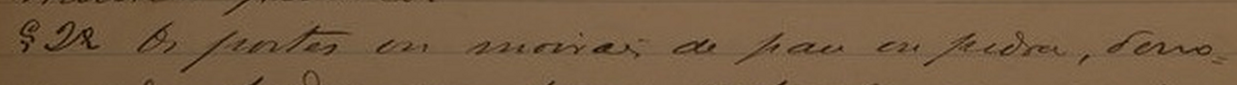
\includegraphics[width=\linewidth]{crops/test10_p22_l029.png}\\[2pt]
{\footnotesize\begin{tabular}{@{}lp{0.68\linewidth}r@{}}
\toprule
referência (normalizada) & º os postes ou moirões de pau ou pedra denominados & erros \\
\midrule
sem pós-correção & § \erro{2º} Os postes ou moirões de pau ou pedra, \erro{deno=} & 2 \\
\textbf{v6 (nossa)} & § \erro{2º} Os postes ou \erro{moitões} de pau ou pedra, \erro{consummados} & 3 \\
A: KenLM & § \erro{28} Os postes ou moirões de pau ou pedra, \erro{donorimados} & 2 \\
B: \textit{word beam} & § \erro{2º} os postes ou moirões de pau ou pedra, \erro{donorimados} & 2 \\
C: ByT5 & § \erro{2.º} Os postes ou moirões de pau ou pedra, \erro{denonumados} & 2 \\
D: v6 + PortOldBERT & § \erro{2º} Os postes ou \erro{moitões} de pau ou pedra, \erro{consummados} & 3 \\
E: VLM & § \erro{2º} Os postes ou moirões de pau ou pedra, \erro{denonmiados} & 2 \\
\bottomrule
\end{tabular}}\\[-2pt]
{\scriptsize página 22 (teste), linha 30}

\noindent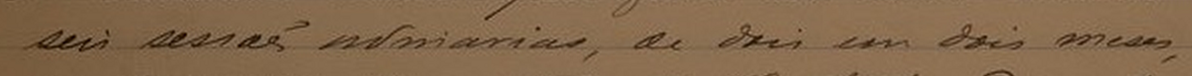
\includegraphics[width=\linewidth]{crops/heldout_p10_l018.png}\\[2pt]
{\footnotesize\begin{tabular}{@{}lp{0.68\linewidth}r@{}}
\toprule
referência (normalizada) & seis sessões ordinarias de dois em dois meses & erros \\
\midrule
sem pós-correção & seis sessões ordinarias, de dois em dois meses, & 0 \\
\textbf{v6 (nossa)} & seis sessões ordinarias, de dois em dois \erro{mezes,} & 1 \\
A: KenLM & seis sessões ordinarias, de dois em dois \erro{mezes,} & 1 \\
B: \textit{word beam} & seis sessões ordinarias, de dois em dois meses, & 0 \\
C: ByT5 & seis sessões ordinarias, de dois em dois \erro{mezes,} & 1 \\
D: v6 + PortOldBERT & seis sessões ordinarias, de dois em dois \erro{mezes,} & 1 \\
E: VLM & seis sessões \erro{ordinárias,} de dois em dois meses, & 1 \\
\bottomrule
\end{tabular}}\\[-2pt]
{\scriptsize página 10 (reservadas), linha 19}

\noindent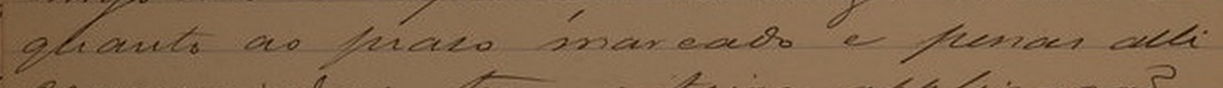
\includegraphics[width=\linewidth]{crops/test10_p24_l010.png}\\[2pt]
{\footnotesize\begin{tabular}{@{}lp{0.68\linewidth}r@{}}
\toprule
referência (normalizada) & quanto ao praso marcado e penas alli comminadas & erros \\
\midrule
sem pós-correção & quanto ao praso marcado e penas alli= & 1 \\
\textbf{v6 (nossa)} & quanto ao praso marcado e penas \erro{communicadas} & 2 \\
A: KenLM & quanto ao praso marcado e penas \erro{allicomminadas} & 2 \\
B: \textit{word beam} & quanto ao praso marcado e penas alli & 1 \\
C: ByT5 & quanto ao praso marcado e penas \erro{allicommunisadas} & 2 \\
D: v6 + PortOldBERT & quanto ao praso marcado e penas \erro{communicadas} & 2 \\
E: VLM & quanto ao \erro{prazo} marcado e penas \erro{alicommunidades} & 3 \\
\bottomrule
\end{tabular}}\\[-2pt]
{\scriptsize página 24 (teste), linha 11}

\noindent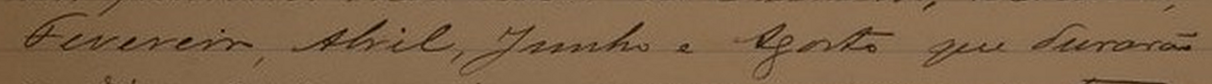
\includegraphics[width=\linewidth]{crops/heldout_p10_l020.png}\\[2pt]
{\footnotesize\begin{tabular}{@{}lp{0.68\linewidth}r@{}}
\toprule
referência (normalizada) & fevereiro abril junho e agosto que durarão & erros \\
\midrule
sem pós-correção & Fevereiro, Abril, Junho e Agosto que durarão & 0 \\
\textbf{v6 (nossa)} & Fevereiro, Abril, \erro{Julho} e Agosto que durarão & 1 \\
A: KenLM & Fevereiro, Abril, Junho e Agosto que durarão & 0 \\
B: \textit{word beam} & fevereiro, abril, junho e agosto que durarão & 0 \\
C: ByT5 & Fevereiro, Abril, Junho e Agosto que durarão & 0 \\
D: v6 + PortOldBERT & Fevereiro, Abril, \erro{Julho} e Agosto que durarão & 1 \\
E: VLM & Fevereiro, Abril, Junho e Agosto que durarão & 0 \\
\bottomrule
\end{tabular}}\\[-2pt]
{\scriptsize página 10 (reservadas), linha 21}

